\documentclass[manuscript,screen,review,acmtog]{acmart}

\citestyle{acmauthoryear}


\begin{document}

\title{Tackling the curse of dimensionality one dimension at a time}

%%
%% The "author" command and its associated commands are used to define
%% the authors and their affiliations.
%% Of note is the shared affiliation of the first two authors, and the
%% "authornote" and "authornotemark" commands
%% used to denote shared contribution to the research.
\author{Yon Ploj}
\email{yp09764@student.uni-lj.si}
\affiliation{%
  \institution{Univerza v Ljubljani, fakulteta za računalništvo in informatiko}
  \city{Ljubljana}
  \country{Slovenia}
}

\renewcommand{\shortauthors}{Ploj, Y.}

\begin{abstract}
This paper presents an implementation and evaluation of Stochastic Dimension Gradient Descent (SDGD)
for solving high-dimensional Black-Scholes partial differential equations using
Physics-Informed Neural Networks (PINNs).
We demonstrate that SDGD significantly accelerates training by reducing the
computational complexity of gradient calculations, particularly in high-dimensional scenarios.
Our experiments show that using a smaller dimension batch size leads to faster learning
while maintaining solution accuracy. We successfully solve problems with up to 100 assets,
achieving substantial speedup compared to traditional approaches.
\end{abstract}

%%
%% The code below is generated by the tool at http://dl.acm.org/ccs.cfm.
%% Please copy and paste the code instead of the example below.
%%
\begin{CCSXML}
<ccs2012>
<concept>
<concept_id>10010147.10010257.10010282.10010283</concept_id>
<concept_desc>Computing methodologies~Batch learning</concept_desc>
<concept_significance>500</concept_significance>
</concept>
<concept>
<concept_id>10010147.10010257.10010293.10010294</concept_id>
<concept_desc>Computing methodologies~Neural networks</concept_desc>
<concept_significance>500</concept_significance>
</concept>
<concept>
<concept_id>10010147.10010257</concept_id>
<concept_desc>Computing methodologies~Machine learning</concept_desc>
<concept_significance>500</concept_significance>
</concept>
</ccs2012>
\end{CCSXML}

\ccsdesc[500]{Computing methodologies~Batch learning}
\ccsdesc[500]{Computing methodologies~Neural networks}
\ccsdesc[500]{Computing methodologies~Machine learning}

\keywords{physics-informed neural networks, stochastic dimension gradient descent, multi-asset Black-Scholes, high-dimensional PDEs}

\received{29 May 2025}
% \received[revised]{12 March 2009}
% \received[accepted]{5 June 2009}

\maketitle

\section{Introduction}
High-dimensional partial differential equations (PDEs) are common in various scientific fields, including (but not limited to) quantum physics, financial mathematics, and climate modelling. However, solving these equations numerically poses a significant challenge due to the curse of dimensionality; a phenomenon where the computational complexity grows exponentially with the number of dimensions.

Physics-Informed Neural Networks (PINNs) have emerged as a promising approach for solving PDEs. By modelling the target function with a neural network and plugging it into the differential equation itself, we can leverage automatic gradient calculation to efficiently fit our neural network to the equation without providing supervised data.

However, PINNs also suffer from the curse of dimensionality when applied to high-dimensional problems. The computational cost of calculating gradients increases exponentially with an increasing number of dimensions, making them impractical for large-scale problems.

To address these challenges, \cite{seminal} proposes a method called stochastic dimension gradient descent (SDGD). By stochastically selecting a subset of dimensions to compute each epoch, we speed up gradient calculation at the cost of stability. The tradeoff can be managed by selecting the size of the dimension batch.

In this paper we present an implementation and evaluation of stochastic dimension gradient descent on a high-dimensional multi-asset Black-Scholes PDE as a testing scenario. The multi-asset Black-Scholes (MABS) is a fundamental model in financial mathematics for pricing options on multiple underlying assets. The MABS PDE provides an excellent benchmark for evaluating SDGD, as it allows us to easily scale the problem dimensionality by arbitrarily increasing the number of assets.

We perform parameter optimization to investigate the impact of various SDGD dimension batch sizes on training speed and solution accuracy. We aim to demonstrate the effectiveness of SDGD in accelerating PINN training for high-dimensional PDEs, with a particular focus on the MABS equation.

\section{Related work}
Physics-Informed Neural Networks (PINNs) were first introduced by \cite{PINNs} as a novel approach to solving PDEs using deep learning. This has been a widely influential paper, cited over 14 thousand times, making it the most cited numerical methods paper of the 21st century.

The curse of dimensionality in PINNs has been addressed through various approaches. Stochastic Dimension Gradient Descent (SDGD) was proposed as a method to reduce computational complexity by randomly sampling dimensions during training by \cite{seminal}. This approach has shown promising results in various high-dimensional PDE problems.

The Black-Scholes equation was first introduced by \cite{bs} as a model for pricing European call options on a single underlying asset. It has since become a cornerstone of financial mathematics, with numerous extensions and applications in the field.

The Black-Scholes model has also been extended to multiple assets by various authors (e.g. \cite{mabs1}, \cite{mabs2}). The multi-asset Black-Scholes PDE incorporates correlation between assets, making it more complex but also more realistic for real-world applications.

\section{Methodology}
Our implementation uses a PINN with a fully connected architecture and configurable hidden dimensions. The network takes $n_{assets} + 1$ input dimensions (asset prices and time) and produces a single output dimension (option price). By default, we use two hidden layers with 16 neurons each.

The neural network architecture consists of:
\begin{itemize}
    \item Input layer: $n_{assets} + 1$ neurons (asset prices and time)
    \item Hidden layer 1: 16 neurons with ReLU activation
    \item Hidden layer 2: 16 neurons with ReLU activation
    \item Output layer: 1 neuron (option price)
\end{itemize}

We initialize the network weights using the Xavier initialization scheme to ensure stable gradient flow during training. The learning rate is set to $10^{-3}$ with an Adam optimizer, which provides good convergence properties for this type of problem.

The training code accepts the number of dimensions to calculate each epoch (dimension batch size). The dimension selection process is implemented using a uniform random sampling without replacement, so that all dimensions are eventually considered.

The loss function incorporates both data and PDE residuals. The loss function is defined as:
\begin{equation}
    L_{total} = \alpha L_{data} + (1-\alpha)L_{pde}
\end{equation}
where $L_{data}$ is the mean squared error on the training data and $L_{pde}$ is the PDE residual loss on randomly sampled collocation points.
The parameter $\alpha$ controls the balance between data fitting and PDE satisfaction. We used $0.1$ in our experiments in order to put a heavy emphasis on learning the PDE, whereas our noisy data serves as more of a guideline.

The PDE residual loss is calculated as:
\begin{equation}
    L_{pde} = \frac{1}{N} \sum_{i=1}^N \left(\frac{\partial V}{\partial t} + \frac{1}{2}\sum_{j=1}^d \sum_{k=1}^d \sigma_j \sigma_k \rho_{jk} S_j S_k \frac{\partial^2 V}{\partial S_j \partial S_k} + r\sum_{j=1}^d S_j \frac{\partial V}{\partial S_j} - rV\right)^2
\end{equation}
where $V$ is the option price, $S_j$ are the asset prices, $\sigma_j$ are the volatilities, $\rho_{jk}$ are the correlation coefficients, and $r$ is the risk-free interest rate.

We ran each experiment for up to an hour. We also implemented an early stopping mechanism to indicate when training has finished, but we found that with a lower dimension batch size, the calculated loss was noisy and unreliable, giving models an unfair advantage. For this reason, we calculated the real loss (on all dimensions) once every 10 seconds, then based our early stopping mechanism on the real loss value.

We evaluated the performance of our implementation on a synthetic dataset.
The generation process consists of two steps. First, we select the data hyperparameters:
\begin{itemize}
    \item Minimum and maximum volatility ($\sigma \in [0.15, 0.35]$)
    \item Minimum and maximum correlation coefficient ($\rho \in [-0.3, 0.7]$)
    \item Minimum and maximum initial asset price ($S_0 \in [15.0, 35.0]$)
    \item Number of data points to generate ($N_{data} = 100$)
    \item Noise variance for the option prices $\sigma_{noise} = 0.1$
\end{itemize}

The data parameters are uniformly sampled from the given ranges.
This hyperparameter preprocessing step is done to ensure that the various assets are not stochastically similar (i.e. we want different price ranges and volatilities for our underlyings).

Then, we simulated correlated Brownian motion paths for each asset, and calculated the final asset prices using geometric Brownian motion.
The option prices are calculated using a basket call option payoff.
Noise is added to the option prices to simulate real-world imperfections.

The generated data finally consists of:
\begin{itemize}
    \item Asset prices ($S$)
    \item Option prices ($C$)
    \item Sampling time points ($t$)
\end{itemize}

The strike price ($K = 20.0$), time to maturity ($T = 1.0$), and risk-free interest rate ($r = 0.035$) are constants.

\section{Evaluation}
We conducted extensive experiments to evaluate the performance of our implementation. The experiments were run on an NVIDIA H100 GPU and covered various combinations of asset counts and dimension batch sizes.
\begin{itemize}
    \item 3 assets, 1 dimension per batch (3-1)
    \item 3 assets, 3 dimensions per batch (3-3)
    \item 30 assets, 1 dimension per batch (30-1)
    \item 30 assets, 10 dimensions per batch (30-10)
    \item 30 assets, 30 dimensions per batch (30-30)
    \item 100 assets, 1 dimension per batch (100-1)
    \item 100 assets, 5 dimensions per batch (100-5)
    \item 100 assets, 100 dimensions per batch (100-100)
\end{itemize}

\begin{figure}
    \centering
    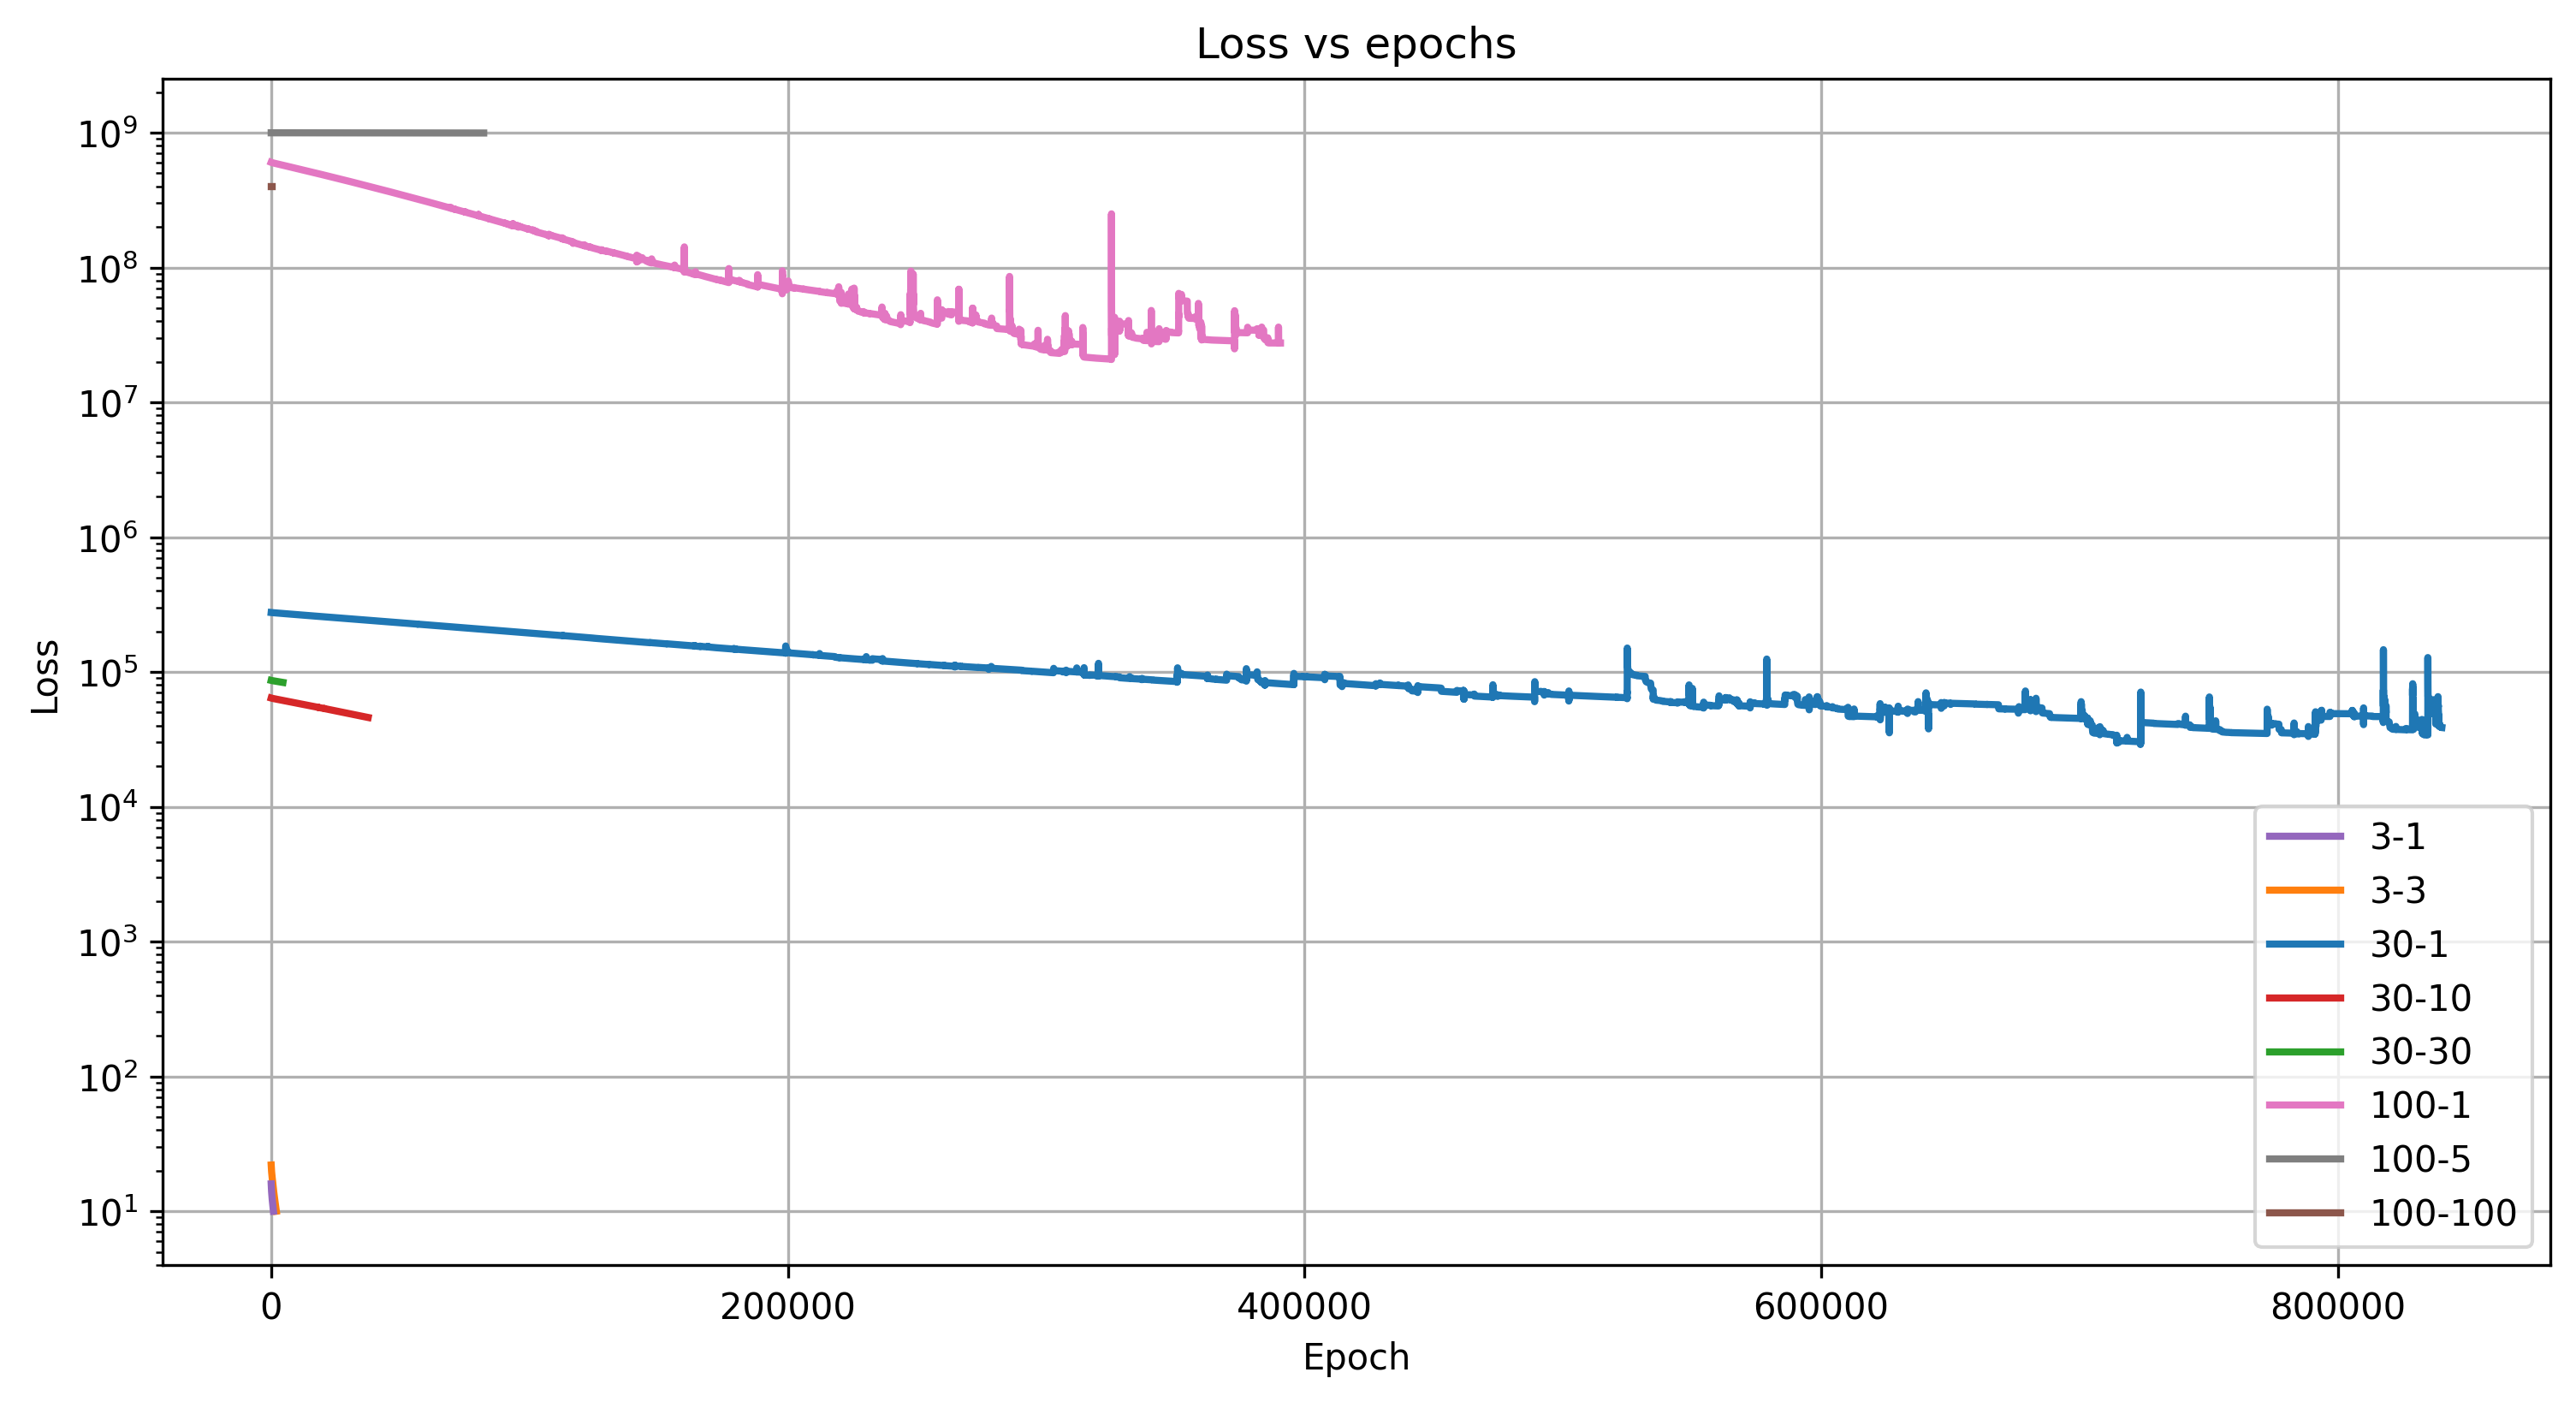
\includegraphics[width=1\linewidth]{loss_vs_epochs.png}
    \caption{Loss vs epochs}
    \label{fig:loss_epochs}
\end{figure}

\begin{figure}
    \centering
    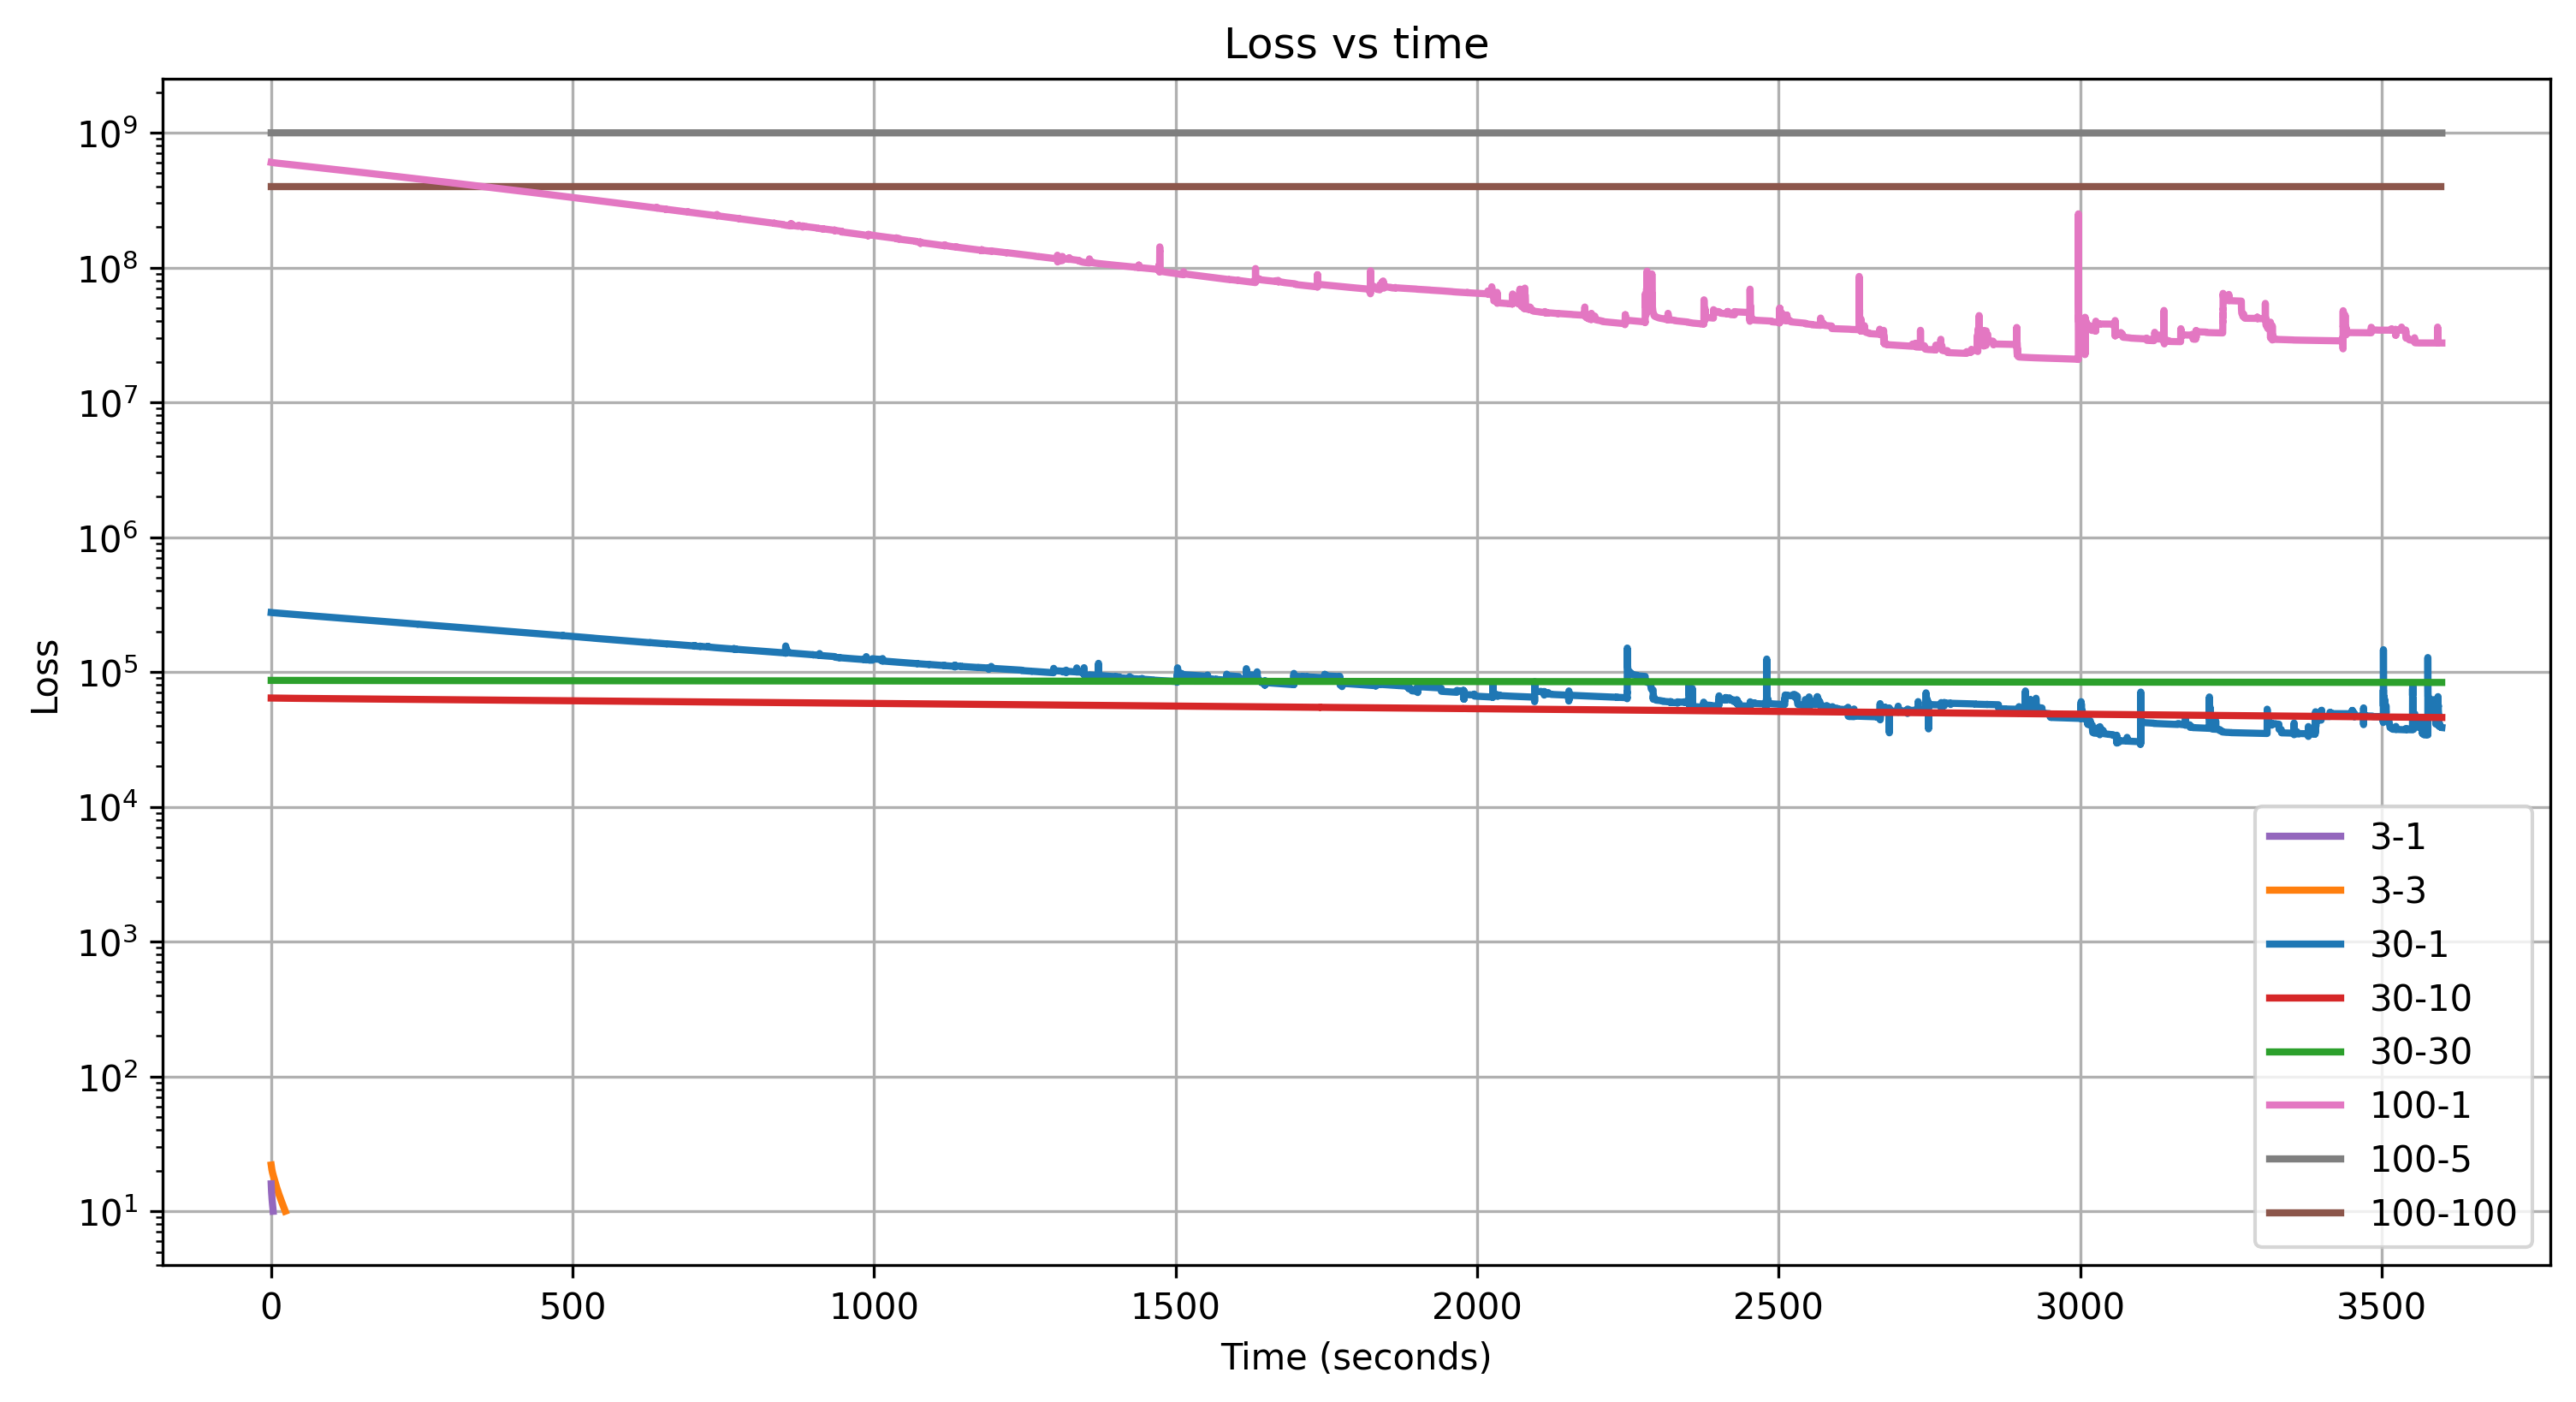
\includegraphics[width=1\linewidth]{loss_vs_time.png}
    \caption{Loss vs time}
    \label{fig:loss_time}
\end{figure}

As seen in figure \ref{fig:loss_time}, smaller dimension batch sizes consistently led to faster learning (indicated by a steeper slope when viewed on a temporal axis), but required more epochs to do so (indicated by a longer running line in figure \ref{fig:loss_epochs}). The most significant improvements were observed in high-dimensional scenarios, as they require the longest processing time per epoch.

The virtually horizontal lines in figure \ref{fig:loss_epochs} indicate the infeasibility of traditional training methods when dealing with a high number of assets. However, SDGD enabled efficient training even with 100 assets.

It is important to note that gradient instability can be a potential drawback when using simplified gradient calculations, as seen in other methods like stochastic gradient descent. Because we did not train our experiments until complete convergence, we cannot discuss the effects of gradient instability, which may cause the network to stop learning before settling into a minimum.

\section{Conclusion}
The results demonstrate that SDGD effectively breaks the curse of dimensionality while maintaining solution quality. The method shows particular promise for high-dimensional problems, where traditional approaches would be computationally infeasible.

We found that smaller dimensions led to faster learning (less real-time until convergence, despite more epochs), even if only using one dimension at a time.

Future work could explore dynamic dimension batch sizing, to provide the optimum in the tradeoff between training speed and gradient stability.

The success of SDGD in solving the multi-asset Black-Scholes PDE suggests that this approach could be valuable for other high-dimensional problems in finance, physics, and other domains where the curse of dimensionality has been a significant barrier.

\bibliographystyle{ACM-Reference-Format}
\bibliography{sample-base}

\appendix

\section{Online Resources}
The implementation and experimental results are available at:\\
https://github.com/plojyon/diffprog-project

\end{document}
\endinput
